\documentclass[11pt]{article}
\usepackage{amsmath, amssymb, amscd, amsthm, amsfonts}
\usepackage{graphicx}
\usepackage{hyperref}
\usepackage{algorithm}
\usepackage{algorithmic}
\usepackage{amsmath}
\usepackage{algorithm}
\usepackage[noend]{algpseudocode}
\usepackage{mathtools}
\usepackage{graphicx}
\graphicspath{ {./images/} }

\newcommand\Myperm[2][^n]{\prescript{#1\mkern-2.5mu}{}P_{#2}}
\newcommand\Mycomb[2][^n]{\prescript{#1\mkern-0.5mu}{}C_{#2}}





 

\oddsidemargin 0pt
\evensidemargin 0pt
\marginparwidth 40pt
\marginparsep 10pt
\topmargin -20pt
\headsep 10pt
\textheight 8.7in
\textwidth 6.65in
\linespread{1.2}

\title{Home work 3}
\author{Vasanth Reddy Baddam}




%\author{Homework by Vasanth Reddy}
\date{02/20/2020}

\newtheorem{theorem}{Theorem}
\newtheorem{lemma}[theorem]{Lemma}
\newtheorem{conjecture}[theorem]{Conjecture}

\newcommand{\rr}{\mathbb{R}}

\newcommand{\al}{\alpha}
\DeclareMathOperator{\conv}{conv}
\DeclareMathOperator{\aff}{aff}

\begin{document}

\maketitle
I pledge that this test/assignment has been completed in compliance with the Graduate Honor Code and
that I have neither given nor received any unauthorized aid on this test/assignment\\
\textbf{Name: } Vasanth Reddy Baddam\\
\textbf{Signature: } VB\\
\hline
\vspace{5mm}
\textbf{Q1.}\\

Given that m = 1000, A = (\sqrt{2} - 1)/2\\
A = (\sqrt{2} - 1)/2 = 0.6180339887....\\

 \begin{tabular}{||c c c c c||} 
 \hline
 \hline
 k &kA& kA mod 1 & m(kA mod 1) & h[k] = \floor*{m(kA mod 1)} \\ [0.5ex] 
 \hline\hline
 32 & 19.77708764 & 0.77708764 & 777.08764 & 777\\ 
 \hline 
 45 & 27.81152949 & 0.81152949 & 811.52949 & 811\\
 \hline
 56 & 34.60990337 & 0.60990337 & 609.90337 & 609\\
 \hline
 62 & 38.31810730 & 0.31810730 & 318.10730 & 318\\
 \hline
 78 & 48.20665112 & 0.20665112 & 206.65112 & 206\\
 \hline 
 90 & 55.62305899 & 0.62305899 & 623.05899 & 623\\[0.2ex]
 \hline
\end{tabular}\\
\vspace{5mm}


\hline

\hline
\vspace{5mm}
\textbf{Q4.}\\
$h(k)$ values for the given are: 5, 1, 1, 6, 2, 6, 3, 8, 1\\
keys 28, 19, and 10 have the same hash function values 1\\
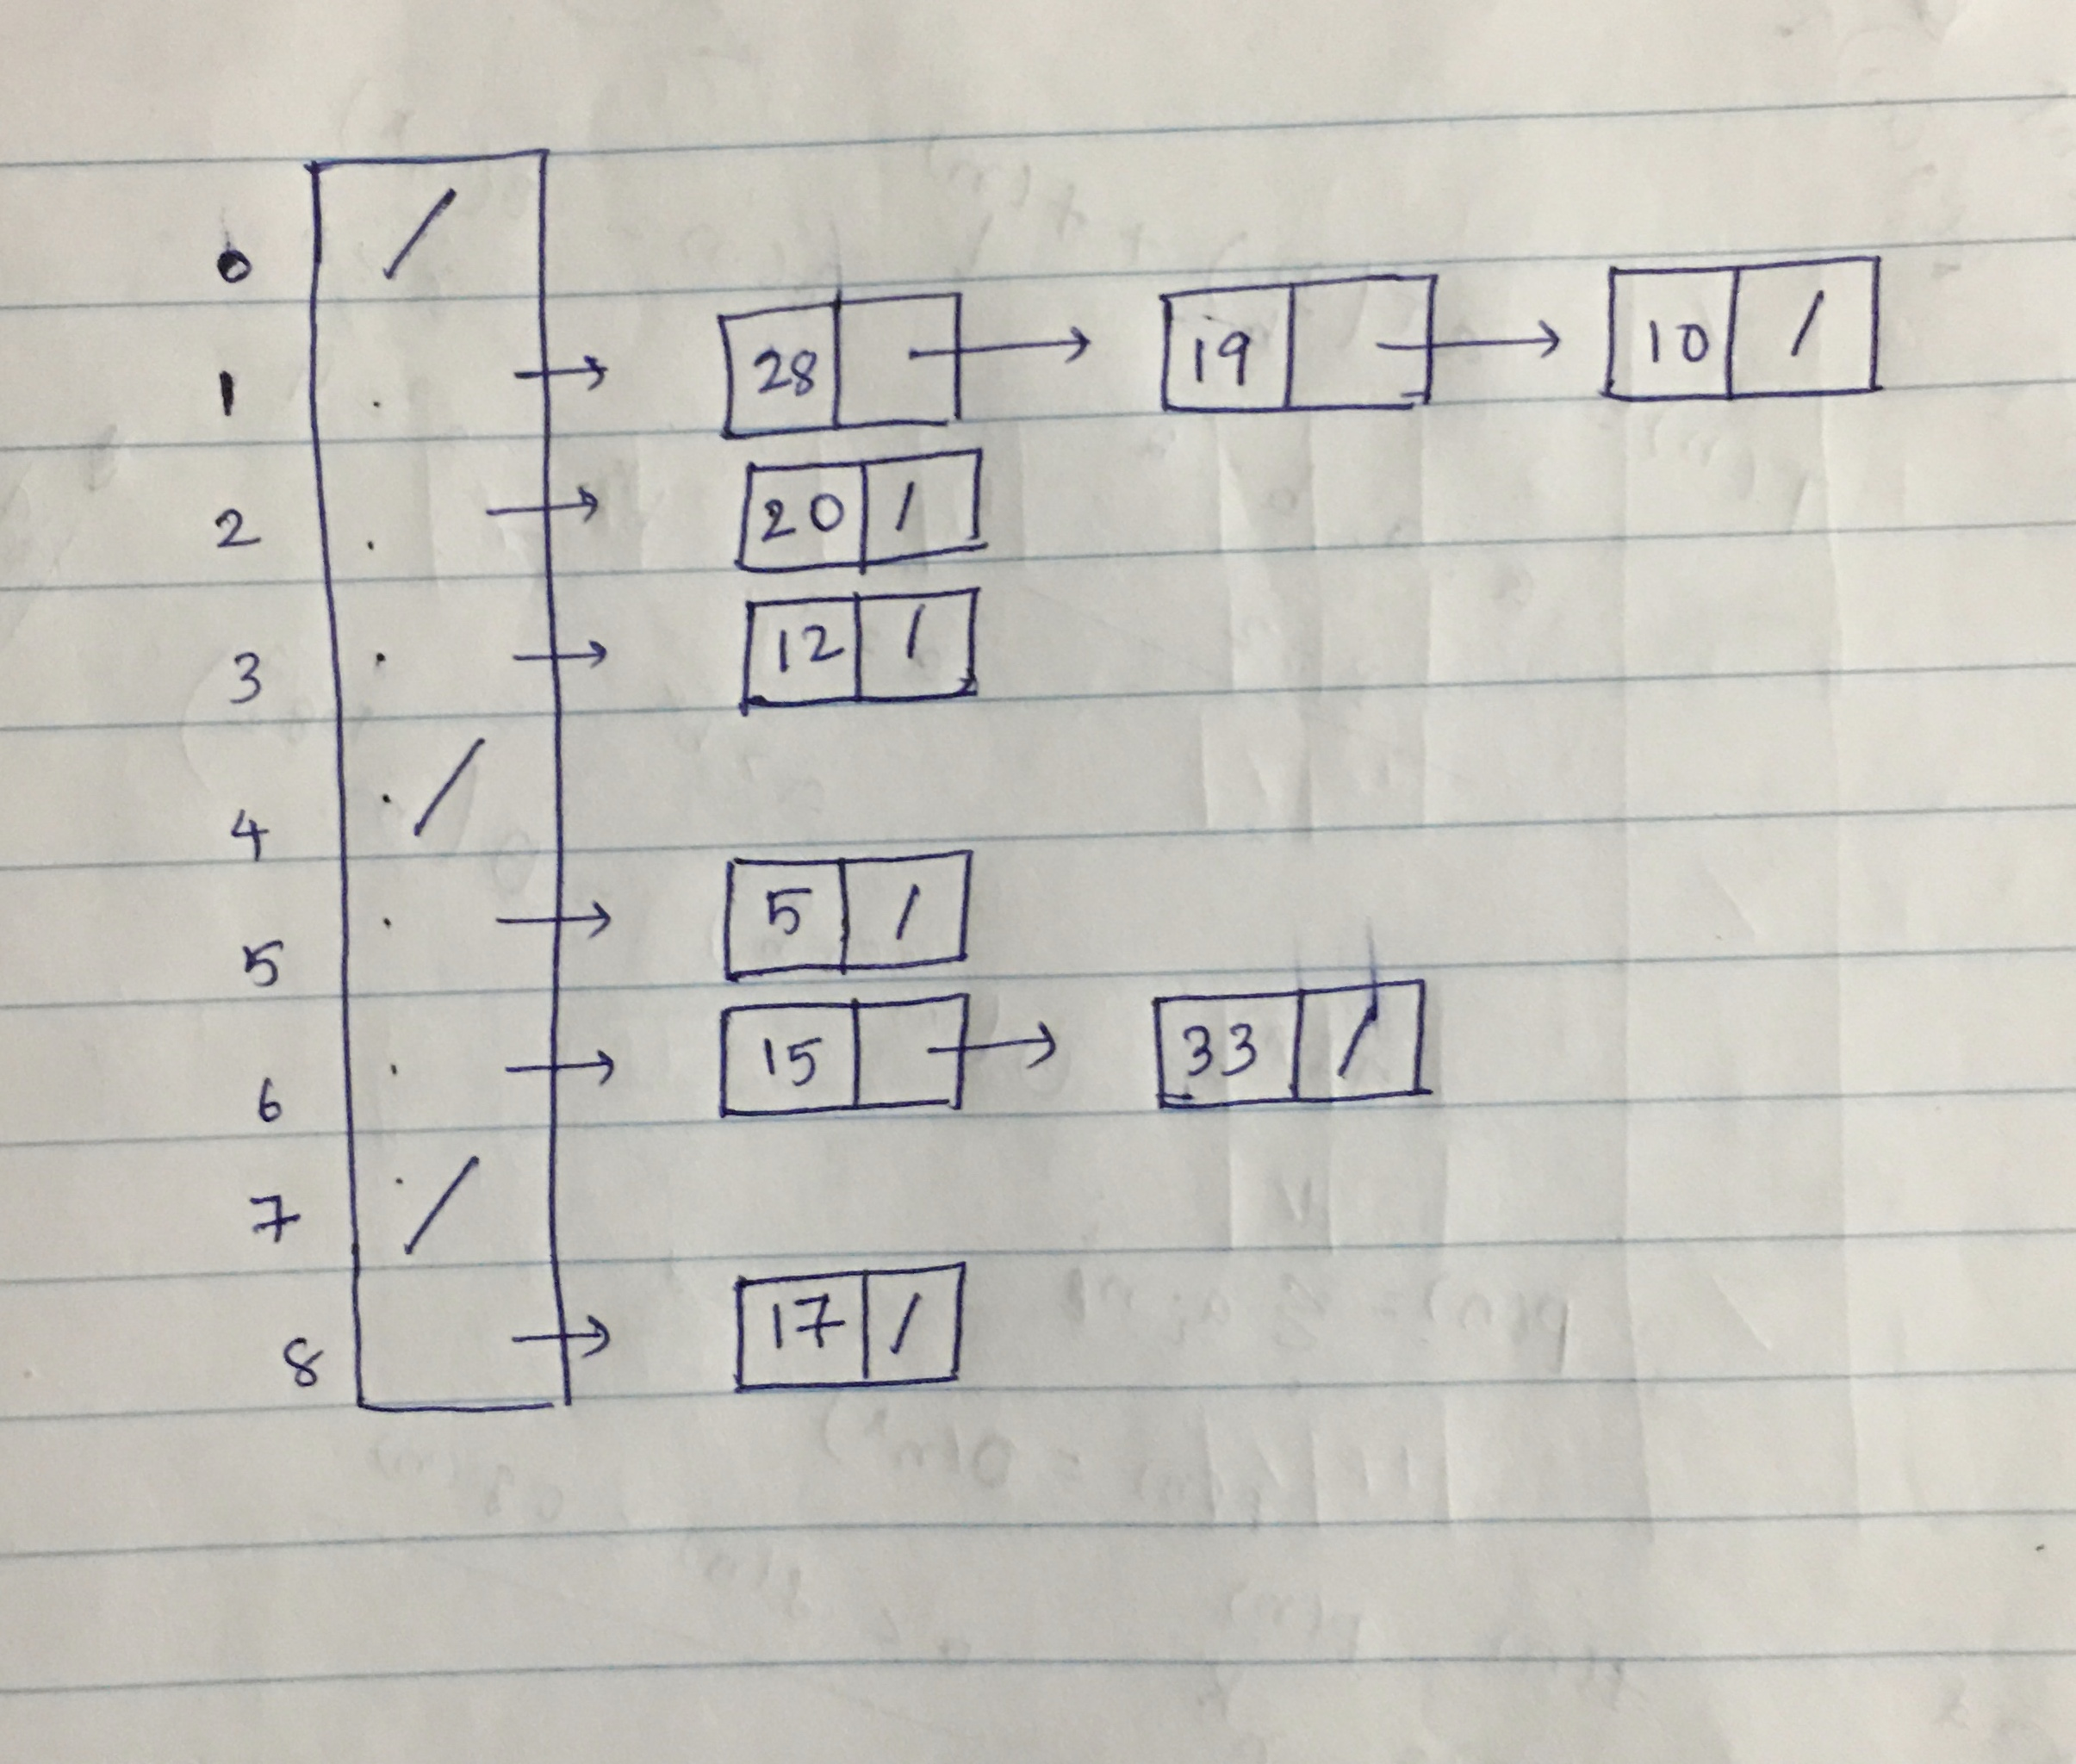
\includegraphics[scale=0.2]{46EE4810-5365-483C-8FC9-DEC8FEAB8562.jpeg}
\vspace{5mm}
\hline
\vspace{5mm}
\textbf{Q3.}\\
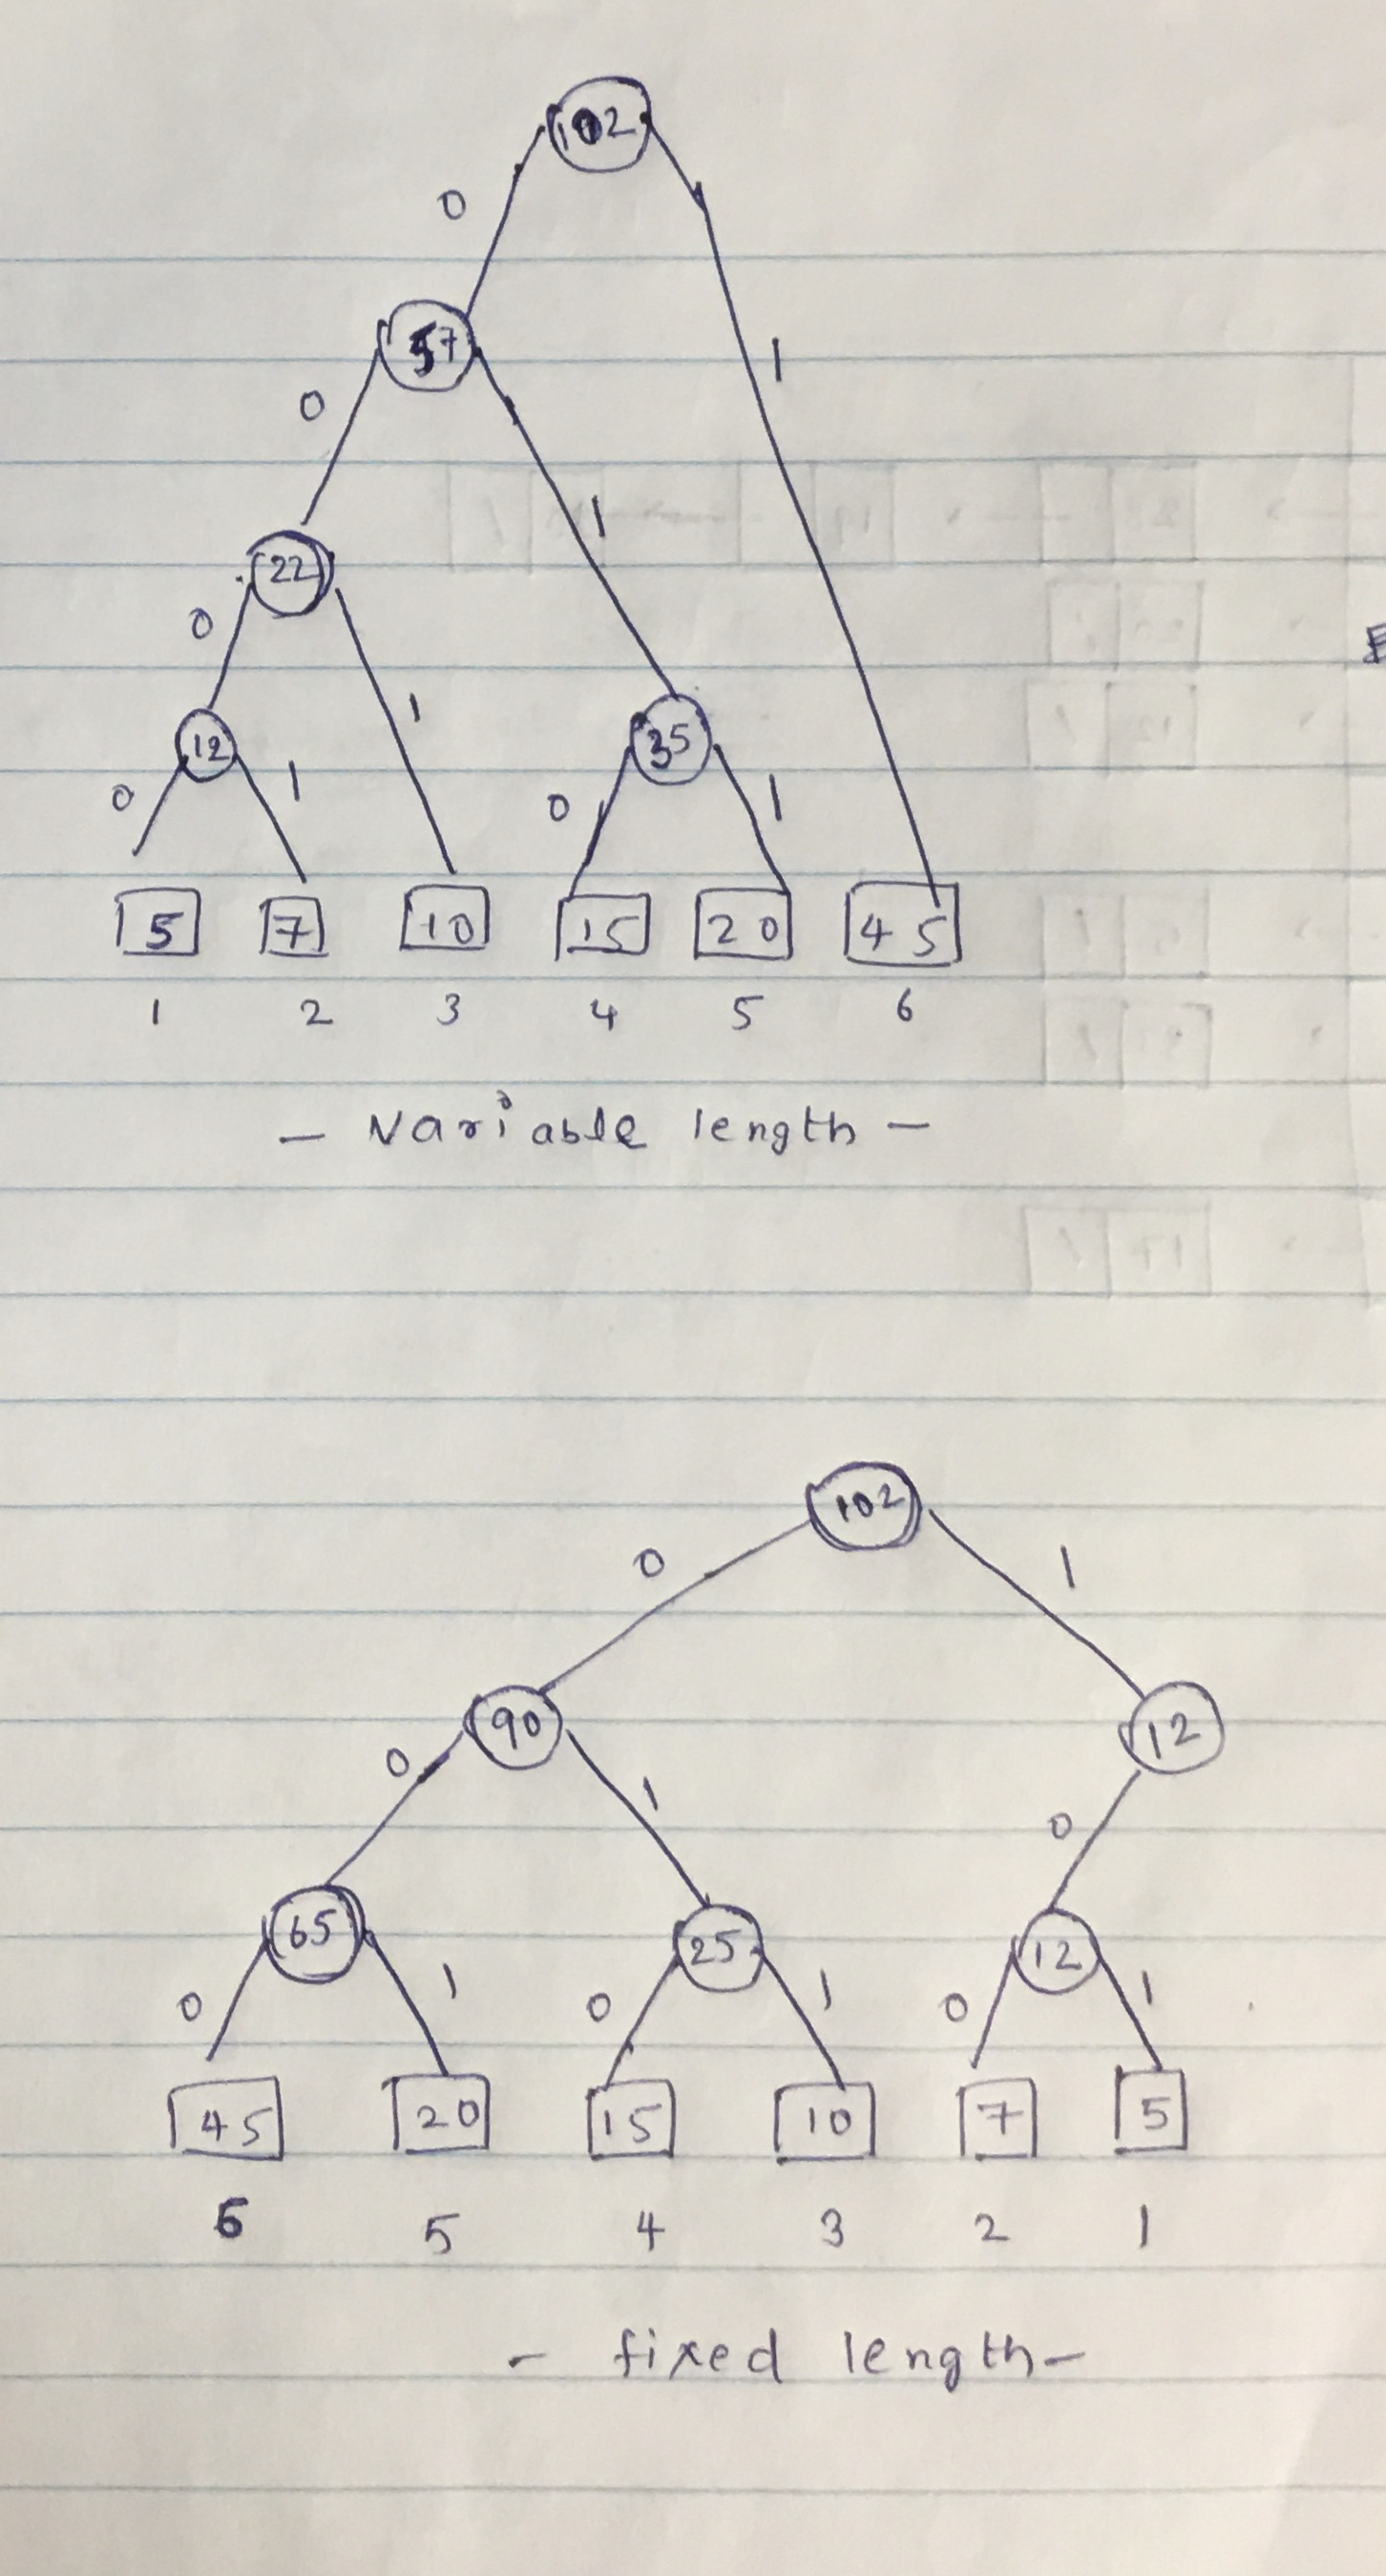
\includegraphics[scale=0.25]{Q3.jpeg}
\begin{center}
 \begin{tabular}{||c c c c c c c c||} 
 \hline
 \hline
   &1& 2 & 3 & 4&5&6&Total bits \\ [0.5ex] 
 \hline\hline
 Frequency& 5 & 7 & 10 &15&20&45&N/A\\ 
 \hline 
 Variable& 0000 & 0001 & 001 & 010&011&1&228\\
 \hline
 Fixed& 101 & 100 & 011 & 010&001&000&306\\[0.2ex]
 \hline
\end{tabular}
\end{center}
\vspace{5mm}
\hline
\vspace{5mm}
\textbf{Q2.}\\
\begin{algorithm}
\caption{Tree Predecessor}\label{euclid}
\begin{algorithmic}
\Procedure{\textsc{Tree-Predecessor}(\textit{x})}{}
\State Set up the environment
\If{x.left $\neq$ NIL} 
\State \textsc{Tree-Maximum}(x.left)
\EndIf
\State y = x.p
\While{y $\neq$ NIL and x == y.left}
\State x = y
\State y = y.p
\EndWhile
\State return(y)
\end{algorithmic}
\end{algorithm}
\vspace{5mm}
\hline
\vspace{5mm}
\textbf{Q5.}\\
\textbf{a).}\\
We have k arrays each having length of $2^i$. where $i$ is the $i$th array.\\
For array of length $n$, running time to search using binary search is $O(\lg{n})$. Worst case would be searching every given array. That is summation of Big O over all the arrays. 

  The worst running time:
  


  \begin{equation}
    \begin{split}
      & \sum_{k=1}^{\lg{n}}{\lg{2^k}}\\
      =& \sum_{k=1}^{\lg{n}}{k}\\
      =& \frac{(1+\lg{n})\times\lg{n}}{2}\\
      =& \frac{\lg^2{n}}{2} + \frac{\lg{n}}{2}
    \end{split}
  \end{equation}

So the worst-case running time is $O(\lg^2{n})$.

\textbf{b).}\\
 Let's say that the element is added in an array. That length will be 1. Then adding this array to $A_0$, then updating the array. Then the obtained array will be merged with $A_1$ and then later updated. This process goes on until all the arrays merges and get updated. This results in $k$ merges. \\
 Worst running would result when all the arrays merge. \\
 Worst running time is $O(2^k)$ as there are $k$ merges.\\
 $$O(2^k) = O(2^{log(n+1)})$$
 $$       = O(n+1)$$
 Worst running time is $O(n)$
\end{document}

